
%% bare_conf.tex
%% V1.4b
%% 2015/08/26
%% by Michael Shell
%% See:
%% http://www.michaelshell.org/
%% for current contact information.
%%
%% This is a skeleton file demonstrating the use of IEEEtran.cls
%% (requires IEEEtran.cls version 1.8b or later) with an IEEE
%% conference paper.
%%
%% Support sites:
%% http://www.michaelshell.org/tex/ieeetran/
%% http://www.ctan.org/pkg/ieeetran
%% and
%% http://www.ieee.org/

%%*************************************************************************
%% Legal Notice:
%% This code is offered as-is without any warranty either expressed or
%% implied; without even the implied warranty of MERCHANTABILITY or
%% FITNESS FOR A PARTICULAR PURPOSE! 
%% User assumes all risk.
%% In no event shall the IEEE or any contributor to this code be liable for
%% any damages or losses, including, but not limited to, incidental,
%% consequential, or any other damages, resulting from the use or misuse
%% of any information contained here.
%%
%% All comments are the opinions of their respective authors and are not
%% necessarily endorsed by the IEEE.
%%
%% This work is distributed under the LaTeX Project Public License (LPPL)
%% ( http://www.latex-project.org/ ) version 1.3, and may be freely used,
%% distributed and modified. A copy of the LPPL, version 1.3, is included
%% in the base LaTeX documentation of all distributions of LaTeX released
%% 2003/12/01 or later.
%% Retain all contribution notices and credits.
%% ** Modified files should be clearly indicated as such, including  **
%% ** renaming them and changing author support contact information. **
%%*************************************************************************


% *** Authors should verify (and, if needed, correct) their LaTeX system  ***
% *** with the testflow diagnostic prior to trusting their LaTeX platform ***
% *** with production work. The IEEE's font choices and paper sizes can   ***
% *** trigger bugs that do not appear when using other class files.       ***                          ***
% The testflow support page is at:
% http://www.michaelshell.org/tex/testflow/



\documentclass[conference]{IEEEtran}
\usepackage{graphicx}
\usepackage{float}

% Some Computer Society conferences also require the compsoc mode option,
% but others use the standard conference format.
%
% If has not been installed into the LaTeX system files,
% manually specify the path to it like:
% \documentclass[conference]{../sty/IEEEtran}





% Some very useful LaTeX packages include:
% (uncomment the ones you want to load)


% *** MISC UTILITY PACKAGES ***
%
%\usepackage{ifpdf}
% Heiko Oberdiek's ifpdf.sty is very useful if you need conditional
% compilation based on whether the output is pdf or dvi.
% usage:
% \ifpdf
%   % pdf code
% \else
%   % dvi code
% \fi
% The latest version of ifpdf.sty can be obtained from:
% http://www.ctan.org/pkg/ifpdf
% Also, note that IEEEtran.cls V1.7 and later provides a builtin
% \ifCLASSINFOpdf conditional that works the same way.
% When switching from latex to pdflatex and vice-versa, the compiler may
% have to be run twice to clear warning/error messages.






% *** CITATION PACKAGES ***
%
\usepackage{cite}
% cite.sty was written by Donald Arseneau
% V1.6 and later of IEEEtran pre-defines the format of the cite.sty package
% \cite{} output to follow that of the IEEE. Loading the cite package will
% result in citation numbers being automatically sorted and properly
% "compressed/ranged". e.g., [1], [9], [2], [7], [5], [6] without using
% cite.sty will become [1], [2], [5]--[7], [9] using cite.sty. cite.sty's
% \cite will automatically add leading space, if needed. Use cite.sty's
% noadjust option (cite.sty V3.8 and later) if you want to turn this off
% such as if a citation ever needs to be enclosed in parenthesis.
% cite.sty is already installed on most LaTeX systems. Be sure and use
% version 5.0 (2009-03-20) and later if using hyperref.sty.
% The latest version can be obtained at:
% http://www.ctan.org/pkg/cite
% The documentation is contained in the cite.sty file itself.






% *** GRAPHICS RELATED PACKAGES ***
%
\ifCLASSINFOpdf
  % \usepackage[pdftex]{graphicx}
  % declare the path(s) where your graphic files are
  % \graphicspath{{../pdf/}{../jpeg/}}
  % and their extensions so you won't have to specify these with
  % every instance of \includegraphics
  % \DeclareGraphicsExtensions{.pdf,.jpeg,.png}
\else
  % or other class option (dvipsone, dvipdf, if not using dvips). graphicx
  % will default to the driver specified in the system graphics.cfg if no
  % driver is specified.
  % \usepackage[dvips]{graphicx}
  % declare the path(s) where your graphic files are
  % \graphicspath{{../eps/}}
  % and their extensions so you won't have to specify these with
  % every instance of \includegraphics
  % \DeclareGraphicsExtensions{.eps}
\fi
% graphicx was written by David Carlisle and Sebastian Rahtz. It is
% required if you want graphics, photos, etc. graphicx.sty is already
% installed on most LaTeX systems. The latest version and documentation
% can be obtained at: 
% http://www.ctan.org/pkg/graphicx
% Another good source of documentation is "Using Imported Graphics in
% LaTeX2e" by Keith Reckdahl which can be found at:
% http://www.ctan.org/pkg/epslatex
%
% latex, and pdflatex in dvi mode, support graphics in encapsulated
% postscript (.eps) format. pdflatex in pdf mode supports graphics
% in .pdf, .jpeg, .png and .mps (metapost) formats. Users should ensure
% that all non-photo figures use a vector format (.eps, .pdf, .mps) and
% not a bitmapped formats (.jpeg, .png). The IEEE frowns on bitmapped formats
% which can result in "jaggedy"/blurry rendering of lines and letters as
% well as large increases in file sizes.
%
% You can find documentation about the pdfTeX application at:
% http://www.tug.org/applications/pdftex





% *** MATH PACKAGES ***
%
\usepackage{amsmath}
% A popular package from the American Mathematical Society that provides
% many useful and powerful commands for dealing with mathematics.
%
% Note that the amsmath package sets \interdisplaylinepenalty to 10000
% thus preventing page breaks from occurring within multiline equations. Use:
%\interdisplaylinepenalty=2500
% after loading amsmath to restore such page breaks as IEEEtran.cls normally
% does. amsmath.sty is already installed on most LaTeX systems. The latest
% version and documentation can be obtained at:
% http://www.ctan.org/pkg/amsmath





% *** SPECIALIZED LIST PACKAGES ***
%
\usepackage{algorithmic}
% algorithmic.sty was written by Peter Williams and Rogerio Brito.
% This package provides an algorithmic environment fo describing algorithms.
% You can use the algorithmic environment in-text or within a figure
% environment to provide for a floating algorithm. Do NOT use the algorithm
% floating environment provided by algorithm.sty (by the same authors) or
% algorithm2e.sty (by Christophe Fiorio) as the IEEE does not use dedicated
% algorithm float types and packages that provide these will not provide
% correct IEEE style captions. The latest version and documentation of
% algorithmic.sty can be obtained at:
% http://www.ctan.org/pkg/algorithms
% Also of interest may be the (relatively newer and more customizable)
% algorithmicx.sty package by Szasz Janos:
% http://www.ctan.org/pkg/algorithmicx




% *** ALIGNMENT PACKAGES ***
%
%\usepackage{array}
% Frank Mittelbach's and David Carlisle's array.sty patches and improves
% the standard LaTeX2e array and tabular environments to provide better
% appearance and additional user controls. As the default LaTeX2e table
% generation code is lacking to the point of almost being broken with
% respect to the quality of the end results, all users are strongly
% advised to use an enhanced (at the very least that provided by array.sty)
% set of table tools. array.sty is already installed on most systems. The
% latest version and documentation can be obtained at:
% http://www.ctan.org/pkg/array


% IEEEtran contains the IEEEeqnarray family of commands that can be used to
% generate multiline equations as well as matrices, tables, etc., of high
% quality.




% *** SUBFIGURE PACKAGES ***
%\ifCLASSOPTIONcompsoc
%  \usepackage[caption=false,font=normalsize,labelfont=sf,textfont=sf]{subfig}
%\else
%  \usepackage[caption=false,font=footnotesize]{subfig}
%\fi
% subfig.sty, written by Steven Douglas Cochran, is the modern replacement
% for subfigure.sty, the latter of which is no longer maintained and is
% incompatible with some LaTeX packages including fixltx2e. However,
% subfig.sty requires and automatically loads Axel Sommerfeldt's caption.sty
% which will override IEEEtran.cls' handling of captions and this will result
% in non-IEEE style figure/table captions. To prevent this problem, be sure
% and invoke subfig.sty's "caption=false" package option (available since
% subfig.sty version 1.3, 2005/06/28) as this is will preserve IEEEtran.cls
% handling of captions.
% Note that the Computer Society format requires a larger sans serif font
% than the serif footnote size font used in traditional IEEE formatting
% and thus the need to invoke different subfig.sty package options depending
% on whether compsoc mode has been enabled.
%
% The latest version and documentation of subfig.sty can be obtained at:
% http://www.ctan.org/pkg/subfig




% *** FLOAT PACKAGES ***
%
%\usepackage{fixltx2e}
% fixltx2e, the successor to the earlier fix2col.sty, was written by
% Frank Mittelbach and David Carlisle. This package corrects a few problems
% in the LaTeX2e kernel, the most notable of which is that in current
% LaTeX2e releases, the ordering of single and double column floats is not
% guaranteed to be preserved. Thus, an unpatched LaTeX2e can allow a
% single column figure to be placed prior to an earlier double column
% figure.
% Be aware that LaTeX2e kernels dated 2015 and later have fixltx2e.sty's
% corrections already built into the system in which case a warning will
% be issued if an attempt is made to load fixltx2e.sty as it is no longer
% needed.
% The latest version and documentation can be found at:
% http://www.ctan.org/pkg/fixltx2e


%\usepackage{stfloats}
% stfloats.sty was written by Sigitas Tolusis. This package gives LaTeX2e
% the ability to do double column floats at the bottom of the page as well
% as the top. (e.g., "\begin{figure*}[!b]" is not normally possible in
% LaTeX2e). It also provides a command:
%\fnbelowfloat
% to enable the placement of footnotes below bottom floats (the standard
% LaTeX2e kernel puts them above bottom floats). This is an invasive package
% which rewrites many portions of the LaTeX2e float routines. It may not work
% with other packages that modify the LaTeX2e float routines. The latest
% version and documentation can be obtained at:
% http://www.ctan.org/pkg/stfloats
% Do not use the stfloats baselinefloat ability as the IEEE does not allow
% \baselineskip to stretch. Authors submitting work to the IEEE should note
% that the IEEE rarely uses double column equations and that authors should try
% to avoid such use. Do not be tempted to use the cuted.sty or midfloat.sty
% packages (also by Sigitas Tolusis) as the IEEE does not format its papers in
% such ways.
% Do not attempt to use stfloats with fixltx2e as they are incompatible.
% Instead, use Morten Hogholm'a dblfloatfix which combines the features
% of both fixltx2e and stfloats:
%
% \usepackage{dblfloatfix}
% The latest version can be found at:
% http://www.ctan.org/pkg/dblfloatfix




% *** PDF, URL AND HYPERLINK PACKAGES ***
%
%\usepackage{url}
% url.sty was written by Donald Arseneau. It provides better support for
% handling and breaking URLs. url.sty is already installed on most LaTeX
% systems. The latest version and documentation can be obtained at:
% http://www.ctan.org/pkg/url
% Basically, \url{my_url_here}.




% *** Do not adjust lengths that control margins, column widths, etc. ***
% *** Do not use packages that alter fonts (such as pslatex).         ***
% There should be no need to do such things with IEEEtran.cls V1.6 and later.
% (Unless specifically asked to do so by the journal or conference you plan
% to submit to, of course. )

\usepackage{subcaption}
\usepackage[utf8]{inputenc}

% correct bad hyphenation here
\hyphenation{op-tical net-works semi-conduc-tor}
\DeclareMathOperator*{\argminA}{arg\,min} % Jan Hlavacek

\begin{document}
%
% paper title
% Titles are generally capitalized except for words such as a, an, and, as,
% at, but, by, for, in, nor, of, on, or, the, to and up, which are usually
% not capitalized unless they are the first or last word of the title.
% Linebreaks \\ can be used within to get better formatting as desired.
% Do not put math or special symbols in the title.
\title{K-Means Algorithm\\and Application in Data Compression\\using Pascal and SwinGame API}

% author names and affiliations
% use a multiple column layout for up to three different
% affiliations
\author{\IEEEauthorblockN{Dung T. Lai}
\IEEEauthorblockA{Faculty of Science, Engineering and Technology\\
Swinburne University of Technology\\
Hawthorn, Victoria 3122\\
Email: tuandunglai@gmail.com}}

% conference papers do not typically use \thanks and this command
% is locked out in conference mode. If really needed, such as for
% the acknowledgment of grants, issue a \IEEEoverridecommandlockouts
% after \documentclass

% for over three affiliations, or if they all won't fit within the width
% of the page, use this alternative format:
% 
%\author{\IEEEauthorblockN{Michael Shell\IEEEauthorrefmark{1},
%Homer Simpson\IEEEauthorrefmark{2},
%James Kirk\IEEEauthorrefmark{3}, 
%Montgomery Scott\IEEEauthorrefmark{3} and
%Eldon Tyrell\IEEEauthorrefmark{4}}
%\IEEEauthorblockA{\IEEEauthorrefmark{1}School of Electrical and Computer Engineering\\
%Georgia Institute of Technology,
%Atlanta, Georgia 30332--0250\\ Email: see http://www.michaelshell.org/contact.html}
%\IEEEauthorblockA{\IEEEauthorrefmark{2}Twentieth Century Fox, Springfield, USA\\
%Email: homer@thesimpsons.com}
%\IEEEauthorblockA{\IEEEauthorrefmark{3}Starfleet Academy, San Francisco, California 96678-2391\\
%Telephone: (800) 555--1212, Fax: (888) 555--1212}
%\IEEEauthorblockA{\IEEEauthorrefmark{4}Tyrell Inc., 123 Replicant Street, Los Angeles, California 90210--4321}}




% use for special paper notices
%\IEEEspecialpapernotice{(Invited Paper)}




% make the title area
\maketitle

% As a general rule, do not put math, special symbols or citations
% in the abstract
\begin{abstract}
Clustering problem is a task of dividing a set of objects (also called members) into different groups (called clusters) based on object's characteristics. Members of a group will have more similarities in comparison with those in other group. This report discusses a traditional clustering method called K-Means algorithm from mathematical perspective. Additionally, an experiment is provided to examine the algorithm in two dimensional space then an application in image compressing.
\end{abstract}

% no keywords




% For peer review papers, you can put extra information on the cover
% page as needed:
% \ifCLASSOPTIONpeerreview
% \begin{center} \bfseries EDICS Category: 3-BBND \end{center}
% \fi
%
% For peerreview papers, this IEEEtran command inserts a page break and
% creates the second title. It will be ignored for other modes.
\IEEEpeerreviewmaketitle


\section{Introduction}
% no \IEEEPARstart
Clustering problems arise in many different applications: machine learning data mining and knowledge discovery, data compression and vector quantization, pattern recognition and pattern classification.~\cite{1}\\
\indent The goal of K-Means Algorithm is to correctly separating objects in a dataset into groups based on object's properties. For instance, objects could be house and their properties are size, number of floor, location, power consumption per year, etc. The goal is to classify house dataset into groups which are luxury, average, poor. In that case, all properties of houses have to be processed to turn into number to create a vector, this process is called vectorization.\\
\indent Another example, take each points in a panel as a objects and each object has two properties which are x-axis and y-axis location. And input $K=3$. The algorithm correctly finds the cluster. (Fig. 1.a)

\begin{figure}[H]
    \centering
    \begin{subfigure}[b]{0.2\textwidth}
        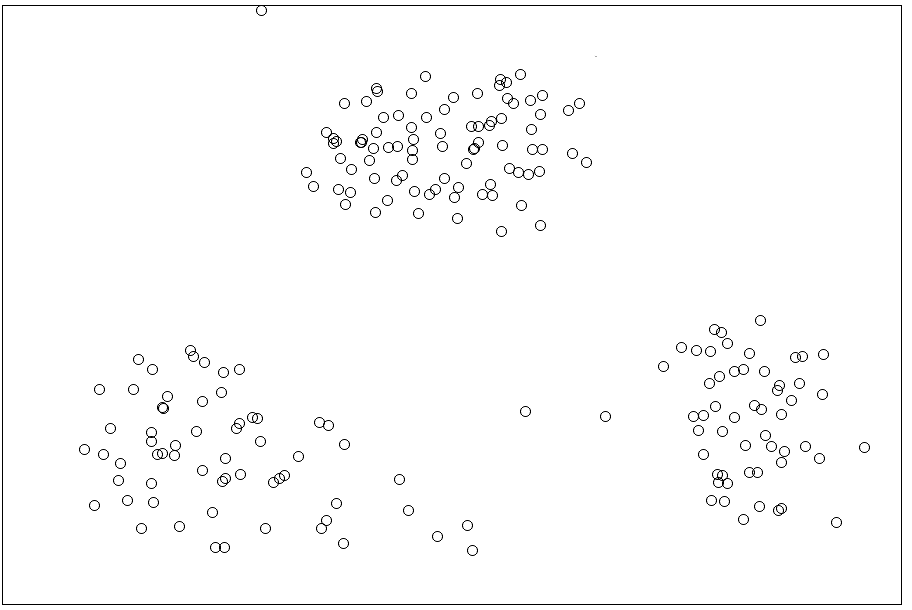
\includegraphics[width=\textwidth]{fig1}
        \caption{Input: $N=200$, $K=3$}
        \label{fig:Input}
    \end{subfigure}
    ~ %add desired spacing between images, e. g. ~, \quad, \qquad, \hfill etc. 
      %(or a blank line to force the subfigure onto a new line)
    \begin{subfigure}[b]{0.2\textwidth}
        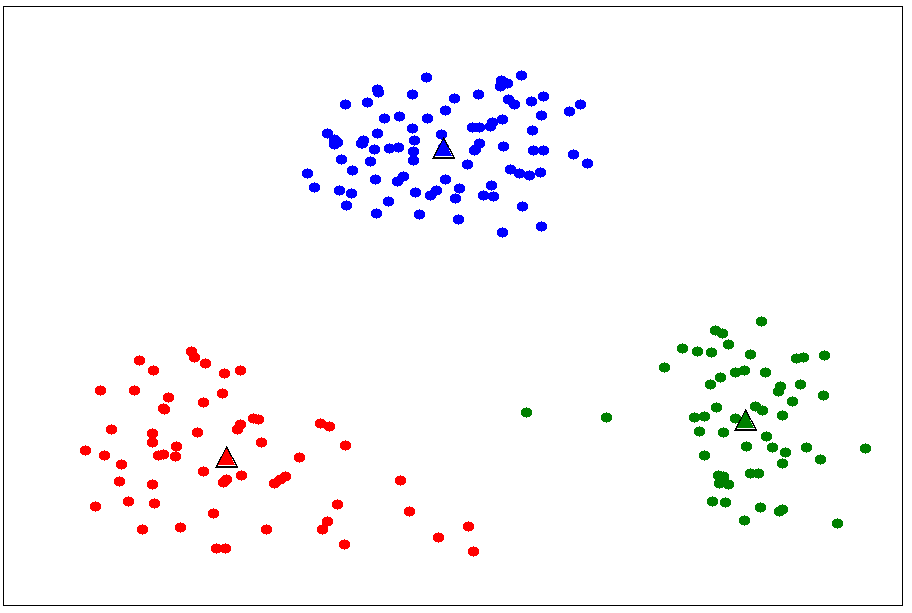
\includegraphics[width=\textwidth]{fig2}
        \caption{Output}
        \label{fig:Output}
    \end{subfigure}
    \caption{K-Means on 2-dimensional Points}
\end{figure}

\section{Mathematical Analysis}
\subsection{Input and Output} \label{input_output}
The K-Means Algorithm takes a set of observations $X=[x_1,x_2,...,x_N]$ $\in$ $R^{d \times N}$ where each observation is a $d$-dimensional vector, $N$ is the number of observations (members) and the number of group $(K, K<N)$ as two input. The algorithm outputs the center of $K$ group $[m_1,m_2,...,m_K] \in R^{d \times K}$ and the index or name of group that each member belonged to (label).
\subsection{Lost Function and Optimization Problem}
Suppose $x_i$ $(i\in[1,N])$ belong to cluster $k$ $(k \in [1,K]$, the lost value of observation $x_i$ is the distance from observation $x_i$ to center $m_k$ in euclidean space, defined by $(x_i-m_k)$.\\
Let's $y_i=[y_{i1},y_{i2},...,y_{iK}]$ be the label vector of each observation $x_i$, $y_{ik}=1$ if $x_i$ belongs to group $k$ and $y_{ij}=0$ $\forall j\neq k$.\\
\indent Label vector of each observation contains only one digit $1$ because each observation belongs to only one group which leads to the following equation.\\
\begin{equation} \label{eq:1}
\sum_{k=1}^{K} y_{ik} = 1
\end{equation}
\indent The objective is to minimize the within-cluster sum of squares (variance), also known as square errors of, where each square error of an observation $x_i$ from group $m_k$ is defined by:
\begin{equation} \label{eq:2}
||x_{i}-m_{k}||^2=y_{ik}||x_{i}-{m_k}||^2
\end{equation}
\indent From the equation \ref{eq:1}, sum of all elements in a label vector is equal 1. The square error of an observation is:
\begin{equation} \label{eq:3}
y_{ik}||x_{i}-{m_k}||^2=\sum_{j=1}^{K}y_{ij}||x_{i}-m_{j}||^2
\end{equation}
\indent The square error of all observation is the sum of every square error of in the given set of observation. The goal is minimize the lost function, equation \ref{eq:4} where $Y=[y_1,y_2,...,y_N]$ be the matrix contains all label vector of $N$ observation and $M=[m_1,m_2,...,m_K]$ be the center of $K$ groups (clusters).
\begin{equation} \label{eq:4}
f(Y,M)=\sum_{i=1}^{N}\sum_{j=1}^{K}y_{ij}||x_i-m_j||^2
\end{equation}
\indent The objective is also to find the center and label vector of each observation which are Y and M, the two outputs that are mentioned in \ref{input_output}. 
\begin{equation} \label{eq:5}
Y,M=argmin_{Y,M}\sum_{i=1}^{N}\sum_{j=1}^{K}y_{ij}||x_i-m_j||^2 
\end{equation}
\subsection{Solving Optimization Problems}
\indent There are two variable in equation \ref{eq:5} which are center of each group of observation and label vector of each observation. The problem could be solved by fixed each variable then minimize the other variable.
\subsubsection{Fixed M, center of observation group} \label{FixedM}
\indent Because all centers ($M$) are constant, the objective is to correctly identify label vector which is identifying the group that each observation belonged to so that the square error in equation \ref{eq:4} is minimized.
\begin{equation} \label{eq:6}
y_i = argmin_{y_i}\sum_{j=1}^{K}y_{ij}||x_i-m_j||^2
\end{equation}
\indent Retrieving from equation \ref{eq:1}. Because only one element in vector $y_i$ $i\in[1,K]=1$. Equation \ref{eq:6} could be rewritten as:
\begin{equation} \label{eq:7}
j=argmin_{j}||x_i-m_j]]^2
\end{equation}
\indent The value of $||x_i-m_j||^2$ is the square of distance from observation to center of group in euclidean space. Concretely, when M is constant, equation \ref{eq:7} shows that minimizing the sum of square error could be achieved by choosing label vector so that the center are closest to observation.
\subsubsection{Fixed Y, label vector of each observation} \label{FixedY}
\indent When label vector ($Y$) are constant, the objective is to correctly identify the center so that the square error in equation \ref{eq:4} is minimized. In this case, the optimization problem in equation \ref{eq:5} could be rewritten by the following equation.
\begin{equation} \label{eq:8}
m_j=argmin_{m_j}\sum_{i=1}^{N}y_{ij}||x_i-m_j||^2
\end{equation}
\indent The equation \ref{eq:8} is a convex function and differentiable for each $i\in[1,N]$. Hence equation \ref{eq:8} could be solved by finding the root of the partial derivative function. This approach will make sure that the root is the the value that make the function reach a optimum.\\
\indent Let's $g(m_j)=\sum_{i=1}^{N}y_{ij}||x_i-m_j||^2$ (retrieving from equation \ref{eq:8} and take the partial derivative of $g(m_j)$:\\
\begin{equation} \label{eq:9}
\frac{\partial g(m_j)}{\partial m_j}=2 \sum_{i=1}^{N}y_{ij}(m_j-x_i)
\end{equation}
\indent The equation \ref{eq:9} is equal 0 is equivalent to:
\begin{equation} \label{eq:10}
m_j\sum_{i=1}^{N}y_{ij}=\sum_{i=1}^{N}y_{ij}x_{i} 
\end{equation}
\begin{equation} \label{eq:11}
\Leftrightarrow m_j=\frac{\sum_{i=1}^{N}y_{ij}x_{i}}{\sum_{i=1}^{N}y_{ij}}
\end{equation}
\indent The value of $y_{ij}=1$ when observation $x_i$ belongs to group $m_j$. Hence, the denominator of equation \ref{eq:11} $\sum_{i=1}^{N}y_{ij}$ is the number of observations that belonging to group $m_j$ and the nominator $\sum_{i=1}^{N}y_{ij}x_{i}$ is the sum of all observations belonging to group $m_j$.\\
\indent In other word, when Y is constant, the square errors could be minimize by assigning the centers to the means of observations in the groups that the observations belonging to.
\subsection{Algorithm summary and Flowchart}
\subsubsection{Summary}
\indent The algorithm can be done by continuously constantize Y and M, one each a time as discussed in \ref{FixedM} and \ref{FixedY}.\\
Step 1.Clusters the data into k groups where k  is predefined.\\
Step 2.Select k points at random as cluster centers.\\
Step 3.Assign objects to their closest cluster center according to the Euclidean distance function.\\
Step 4.Calculate the centroid or mean of all objects in each cluster.\\
Step 5.Repeat steps 2.
\subsubsection{Flowchart}
\indent The following chart describe K-Means Algorithm
\begin{figure}[H]
    \centering
    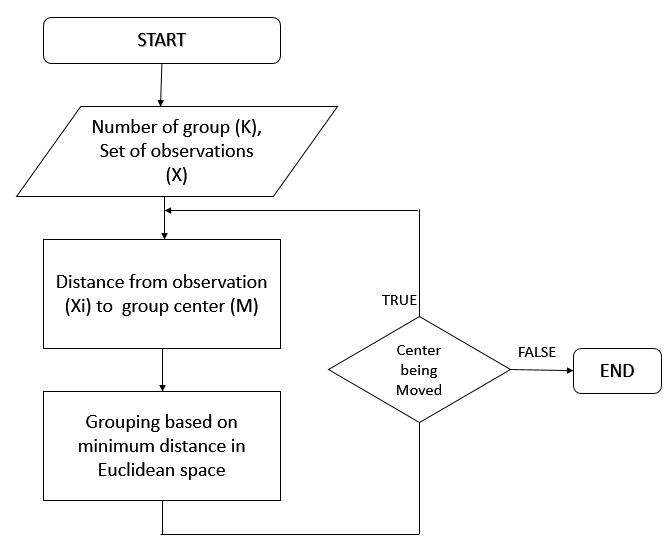
\includegraphics[width=8cm]{fig3}
    \caption{K-Means Algorithm Flowchart}
    \label{fig:fig3}
\end{figure}
\subsection{Discussion}
	\subsubsection{Convergence}
	\indent The algorithm will stop after a certain number of iteration because the square error function is a strictly decreasing sequence and the square error is always greater than 0. But this algorithm will not make sure that it will find a global optimum because solving the equation \ref{eq:8} by finding the root when the partial derivative is equal 0 will only return the value for local optima but not make sure that local optima will be a global minimum. \\
	\indent The following figure describe a case where poorly seeding leads to a local optimum.
\begin{figure}[H]
    \centering
    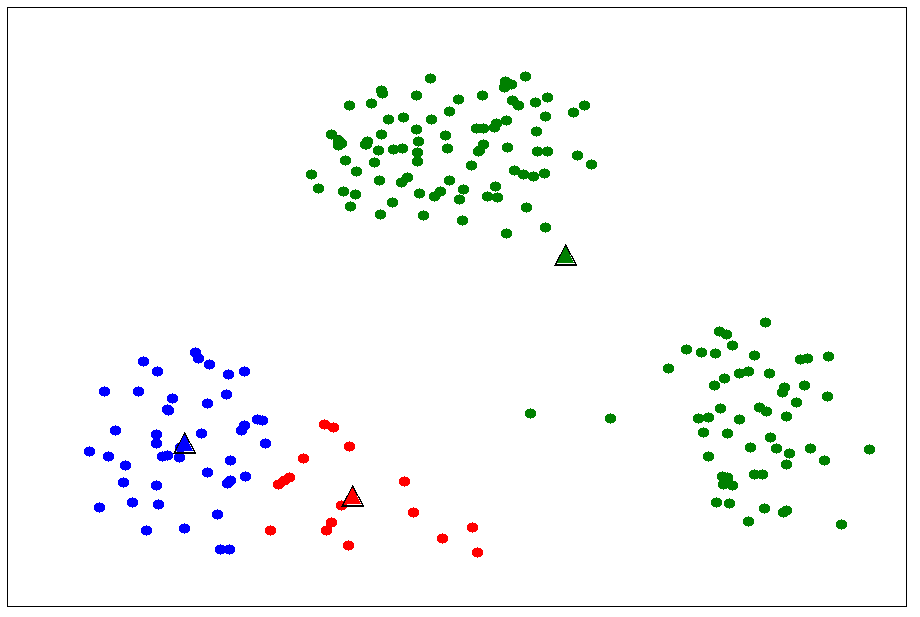
\includegraphics[width=8cm]{fig4}
    \caption{Poorly Seeding K-Means}
    \label{fig:fig4}
\end{figure}
\indent
	In this case, the square error is 6769747 which is about 4 times greater than the square error produce by figure \ref{fig:Output} (1614826).	
	\subsubsection{Sensitiveness to initial cluster}
	\indent K-Means algorithm requires careful seeding, which means the final result is very sensitive to the initial value of cluster. Numerous efforts have been made to improving K-Means clustering algorithm due to its drawbacks ~\cite{2}
\section{Application in Data Compression}
\indent An experiment will be reperformed where K-Means algorithm is applied to reduce the size of image and outputs a new image without the smaller number of color as compared to the original one. This experiment is carried using Pascal programming language and SwinGame API.
\indent Each pixel of a image contains three elements which are red, green, blue (RGB) value. Let's each pixel be the observation ($X$) then the number of pixel in an image be the number of observations. Each observation has three properties which are RGB value. In this case, K-Means algorithm is applied to identify $K$ main colors in that image. \\
\begin{figure}[H]
    \begin{subfigure}[b]{0.23\textwidth}
    	\centering
        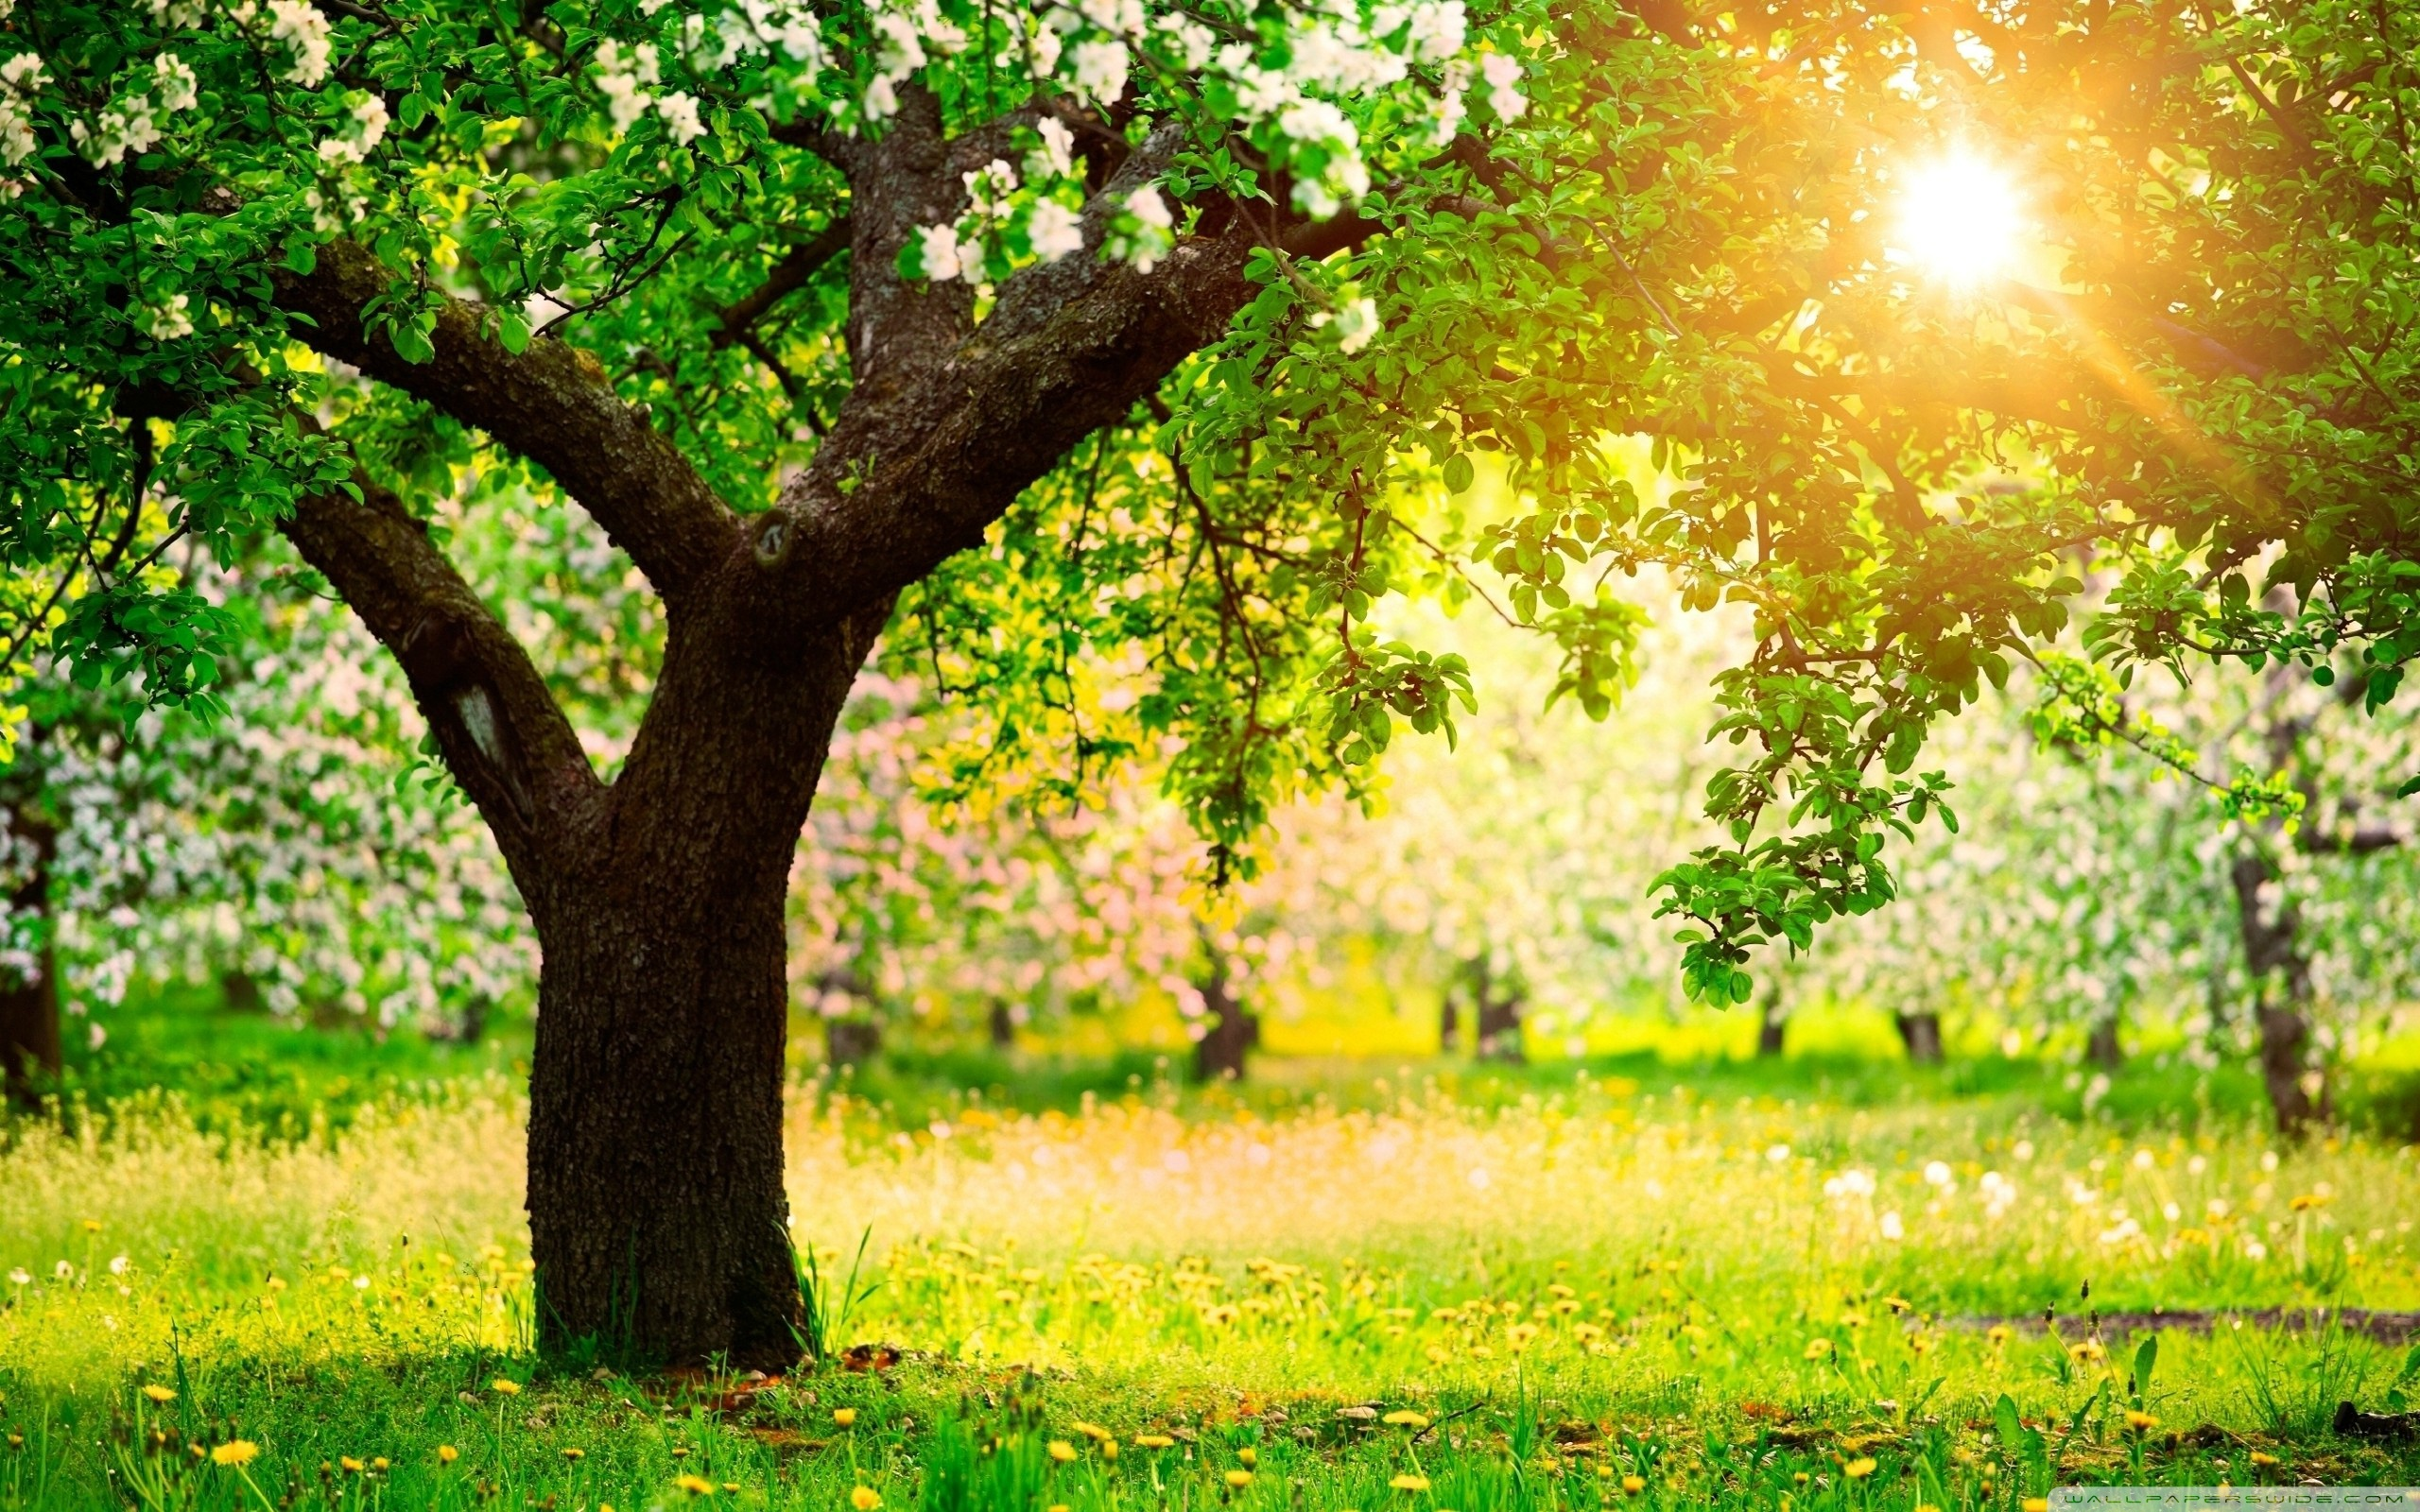
\includegraphics[width=\textwidth]{testx}
        \caption{Original image}
        \label{fig:Input}
    \end{subfigure}
	\hfill
    \begin{subfigure}[b]{0.23\textwidth}
        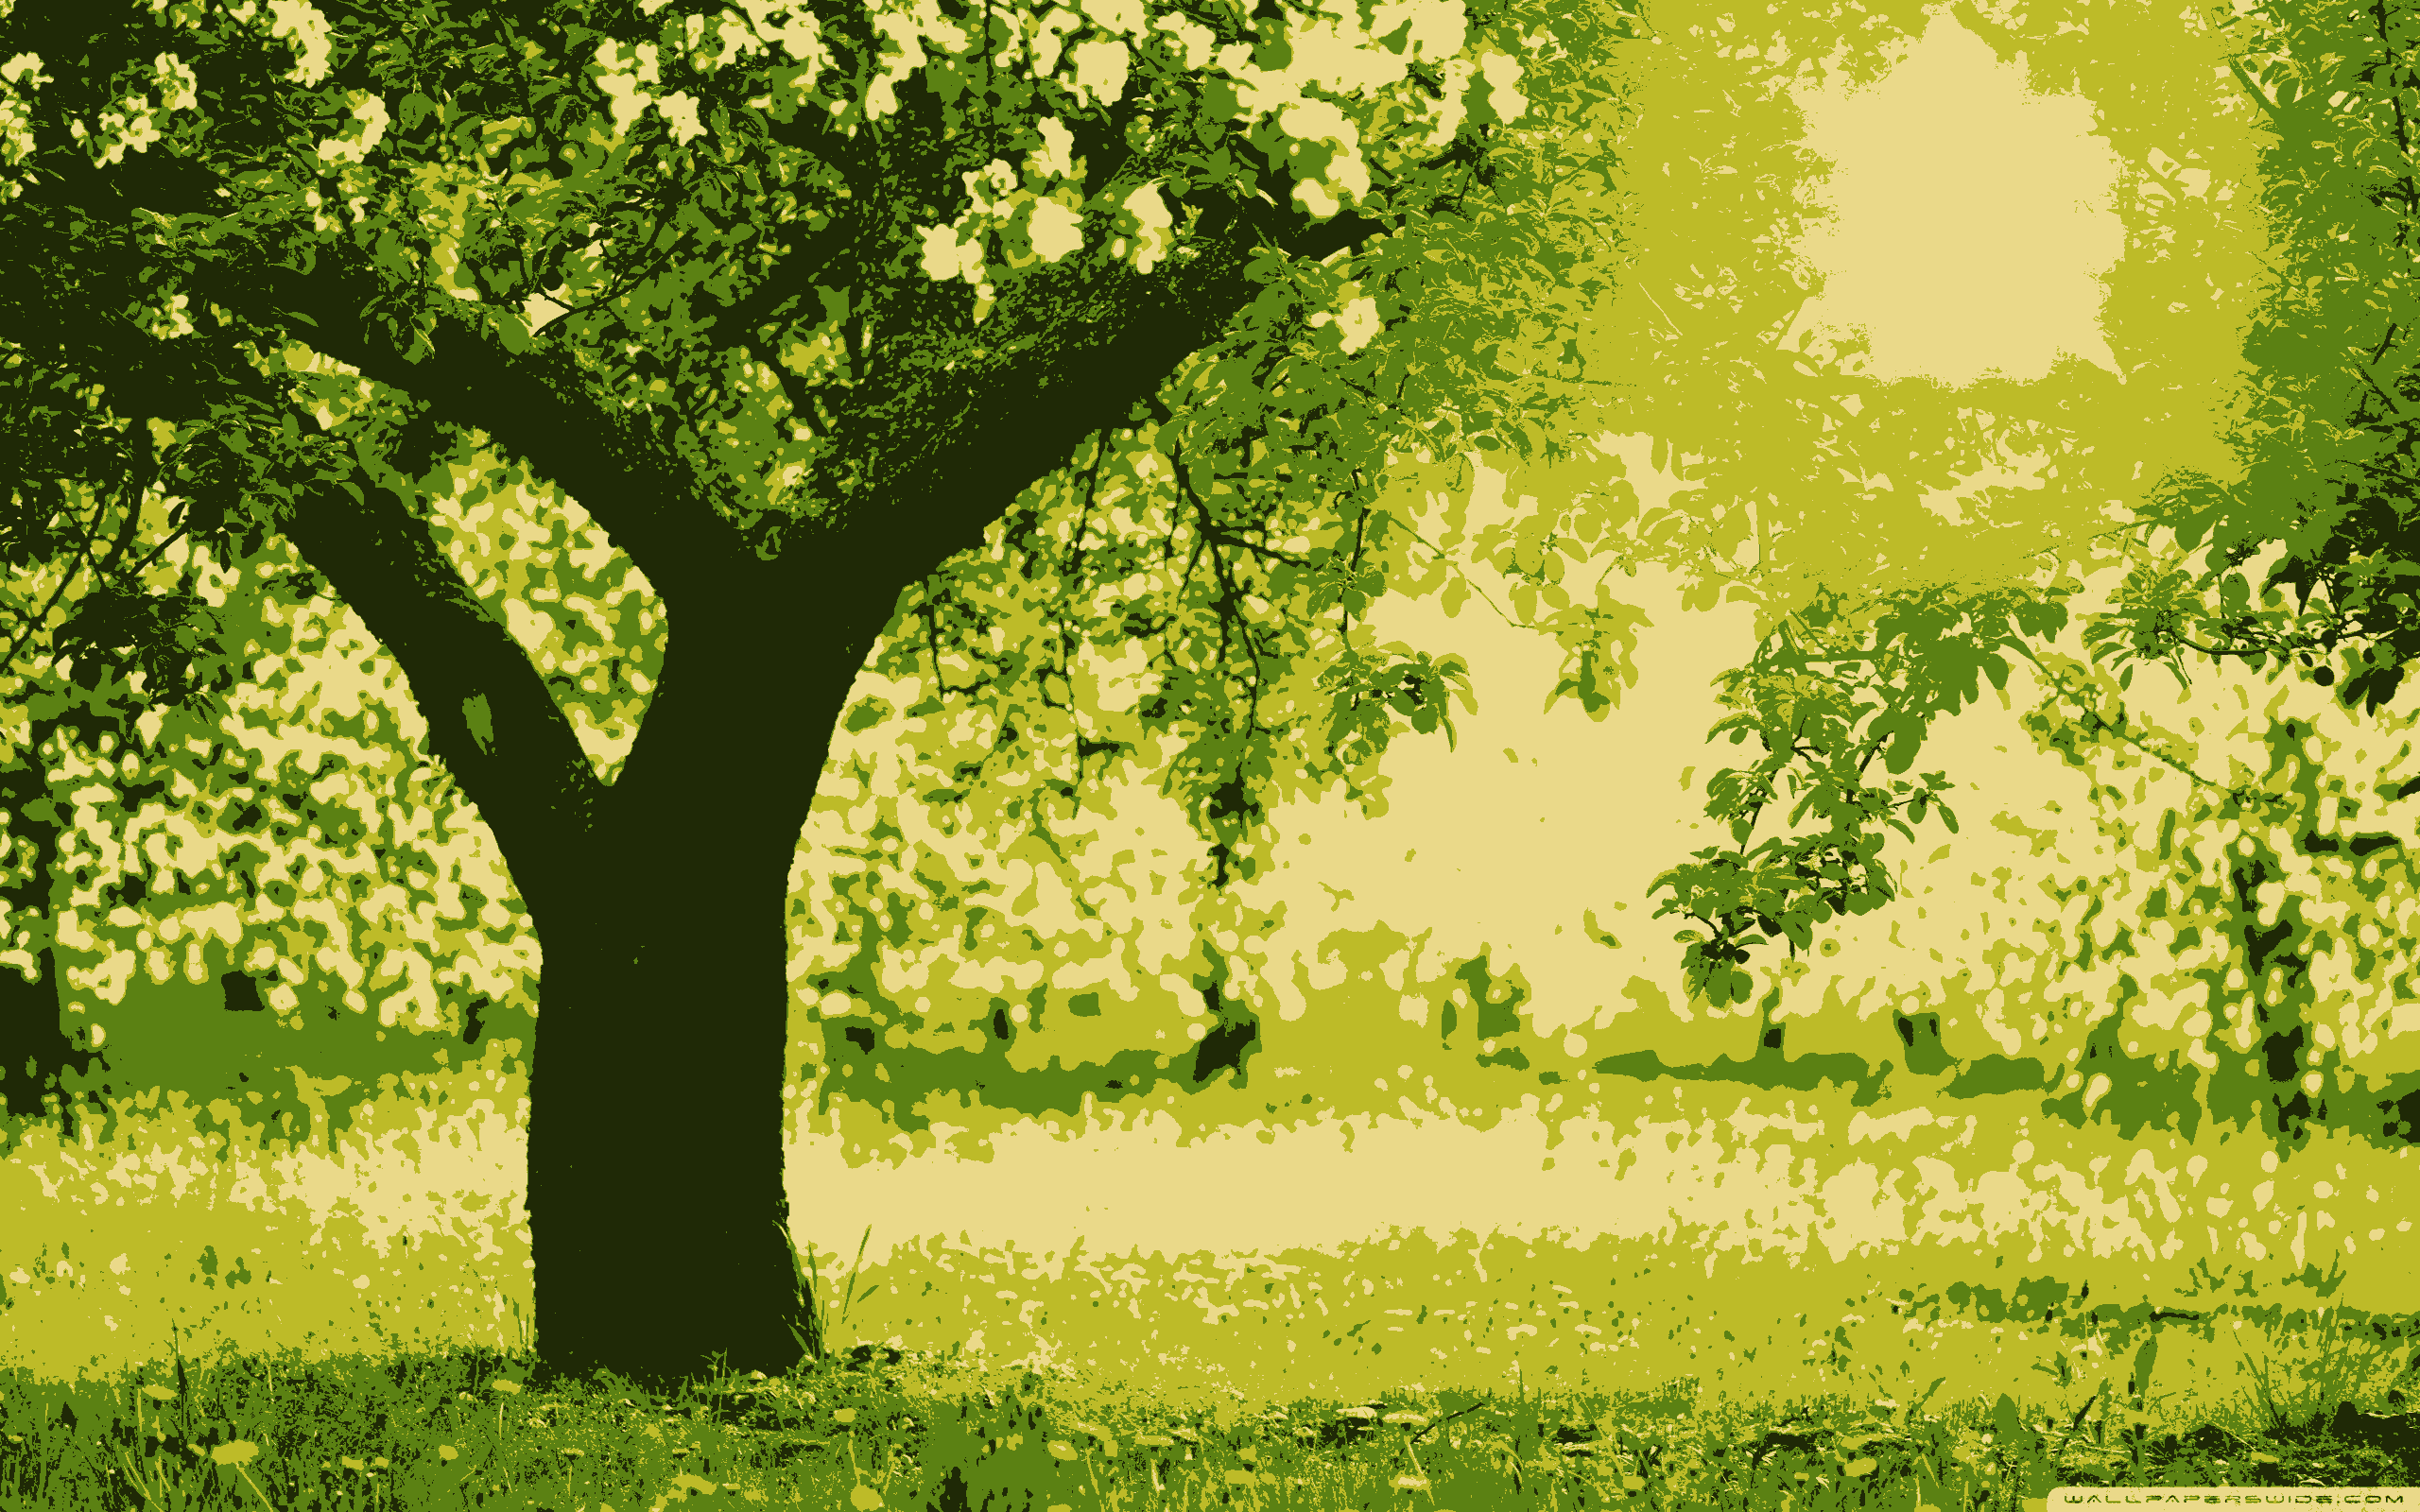
\includegraphics[width=\textwidth]{4Color}
        \caption{$K=4$}
        \label{fig:4Color}
    \end{subfigure}
    \vskip\baselineskip
    \begin{subfigure}[b]{0.23\textwidth}
        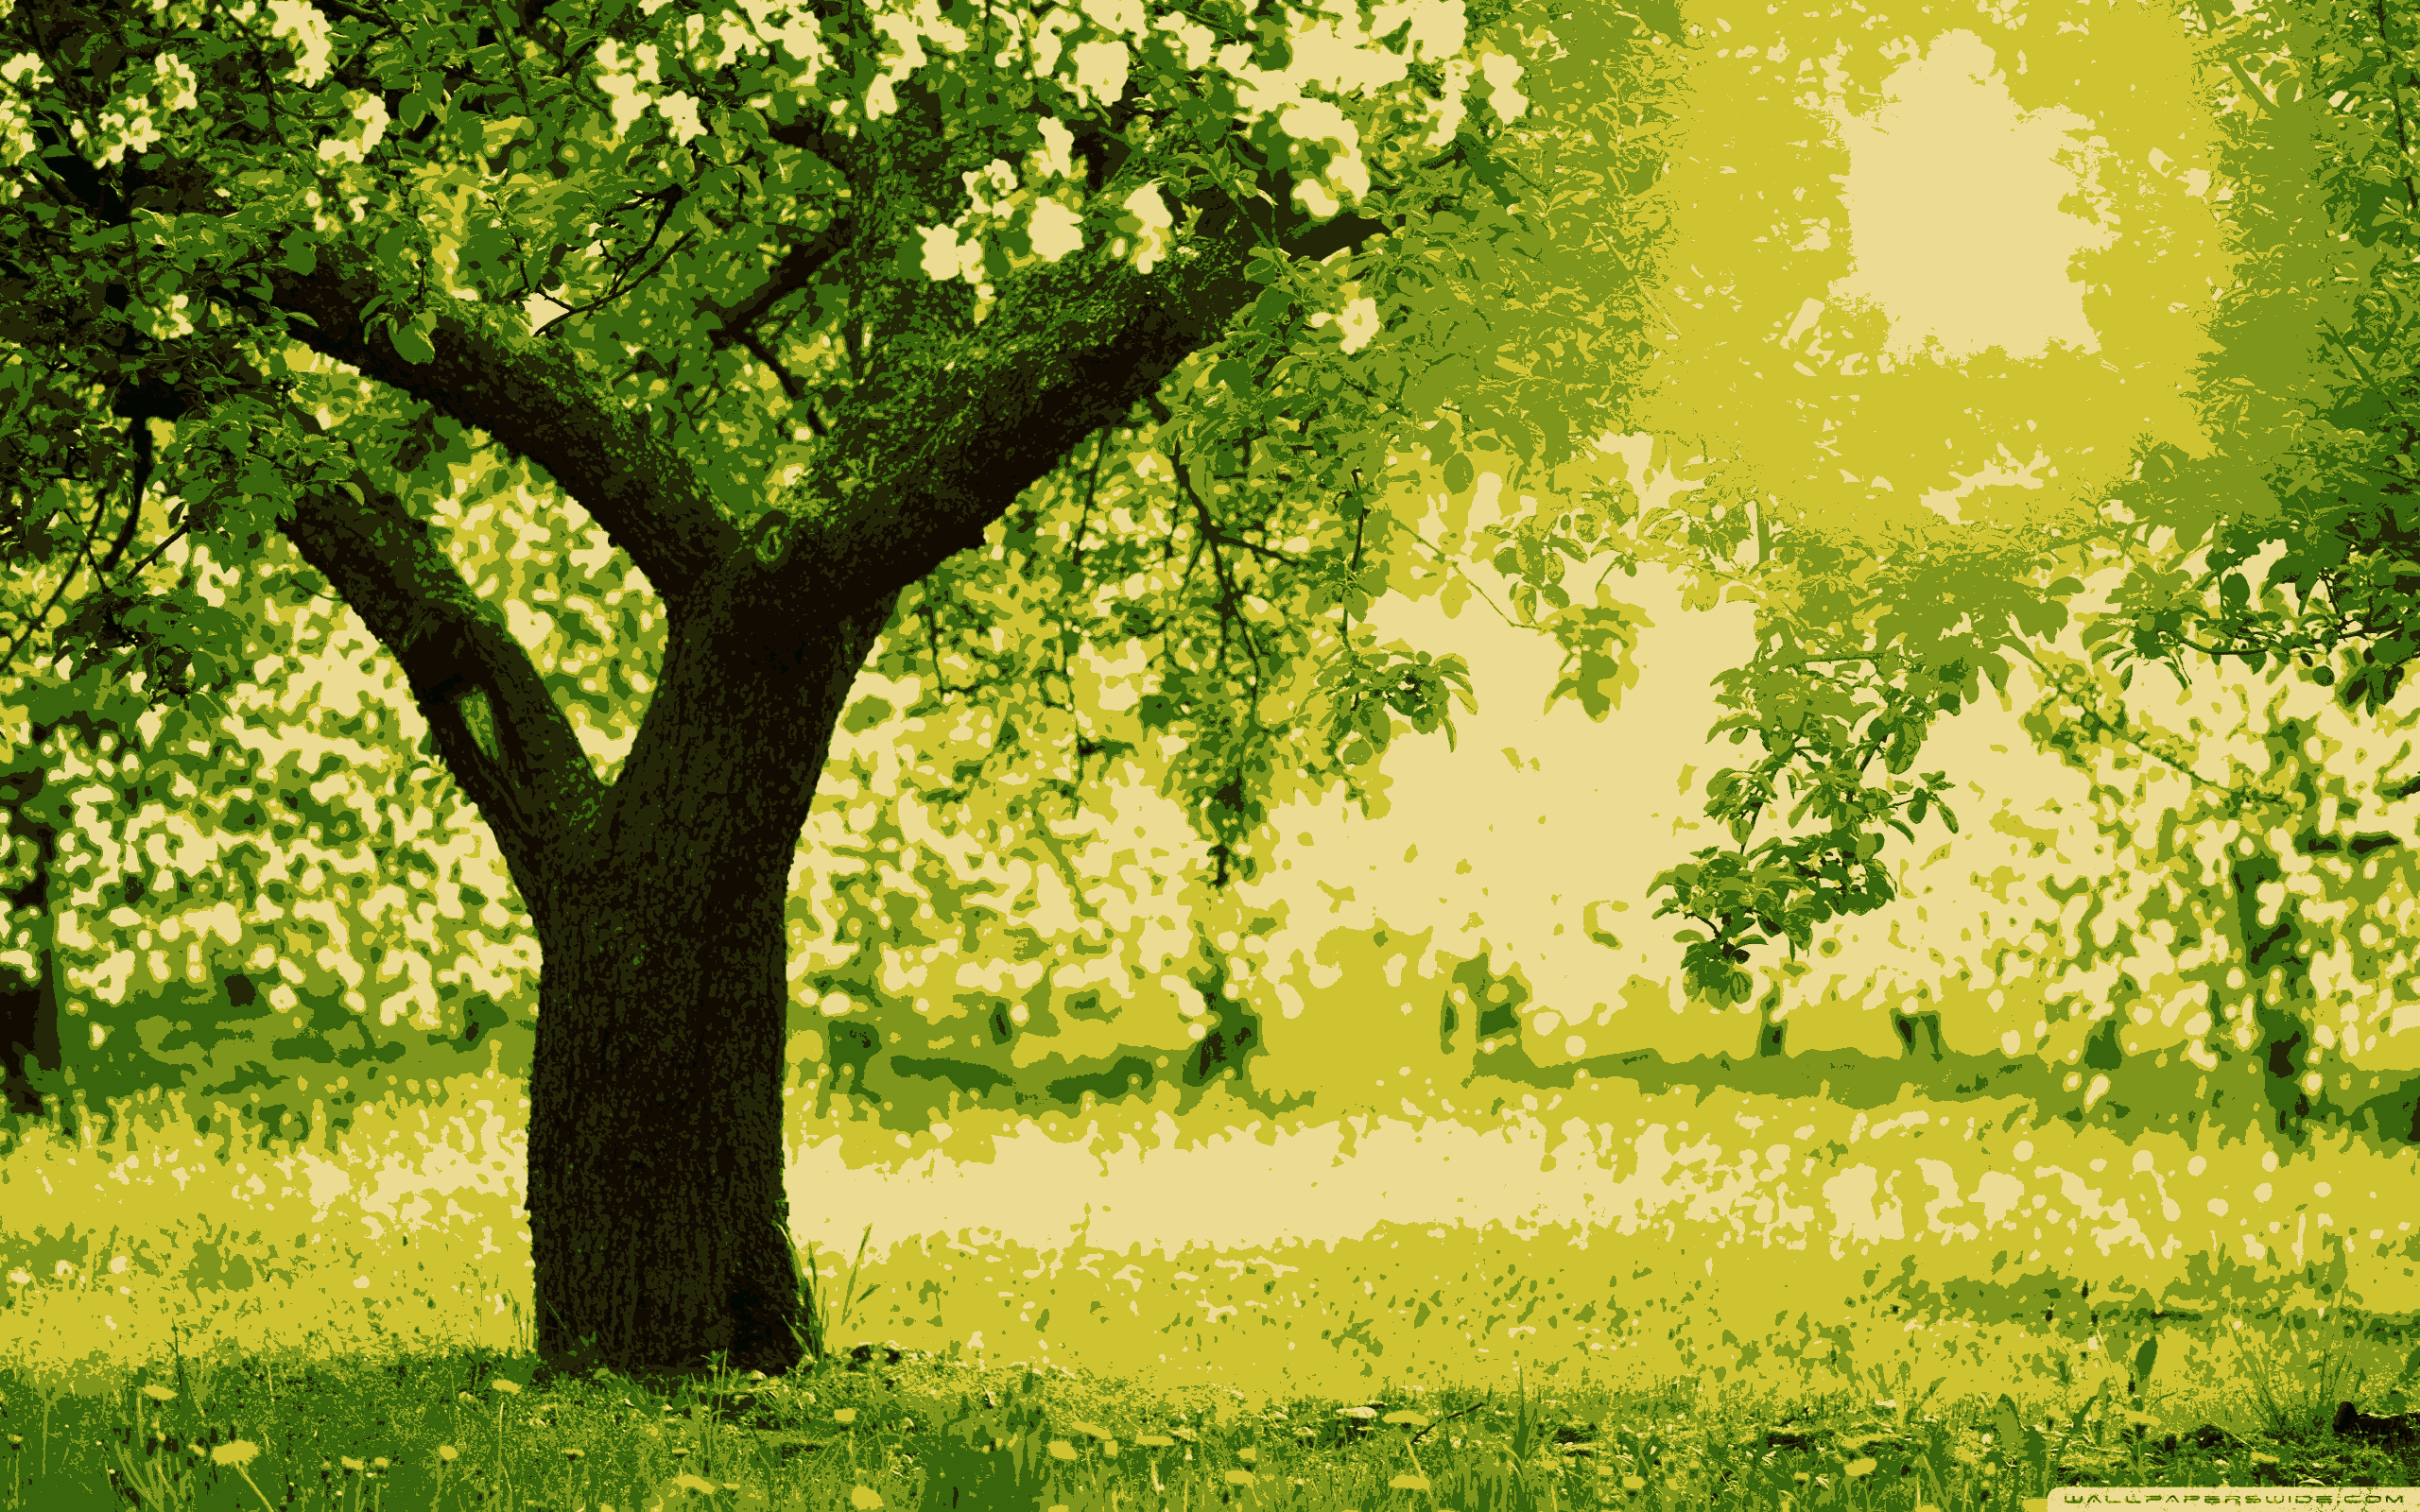
\includegraphics[width=\textwidth]{7Color}
        \caption{$K=7$}
        \label{fig:7Color}
    \end{subfigure}
    \quad
    \begin{subfigure}[b]{0.23\textwidth}
        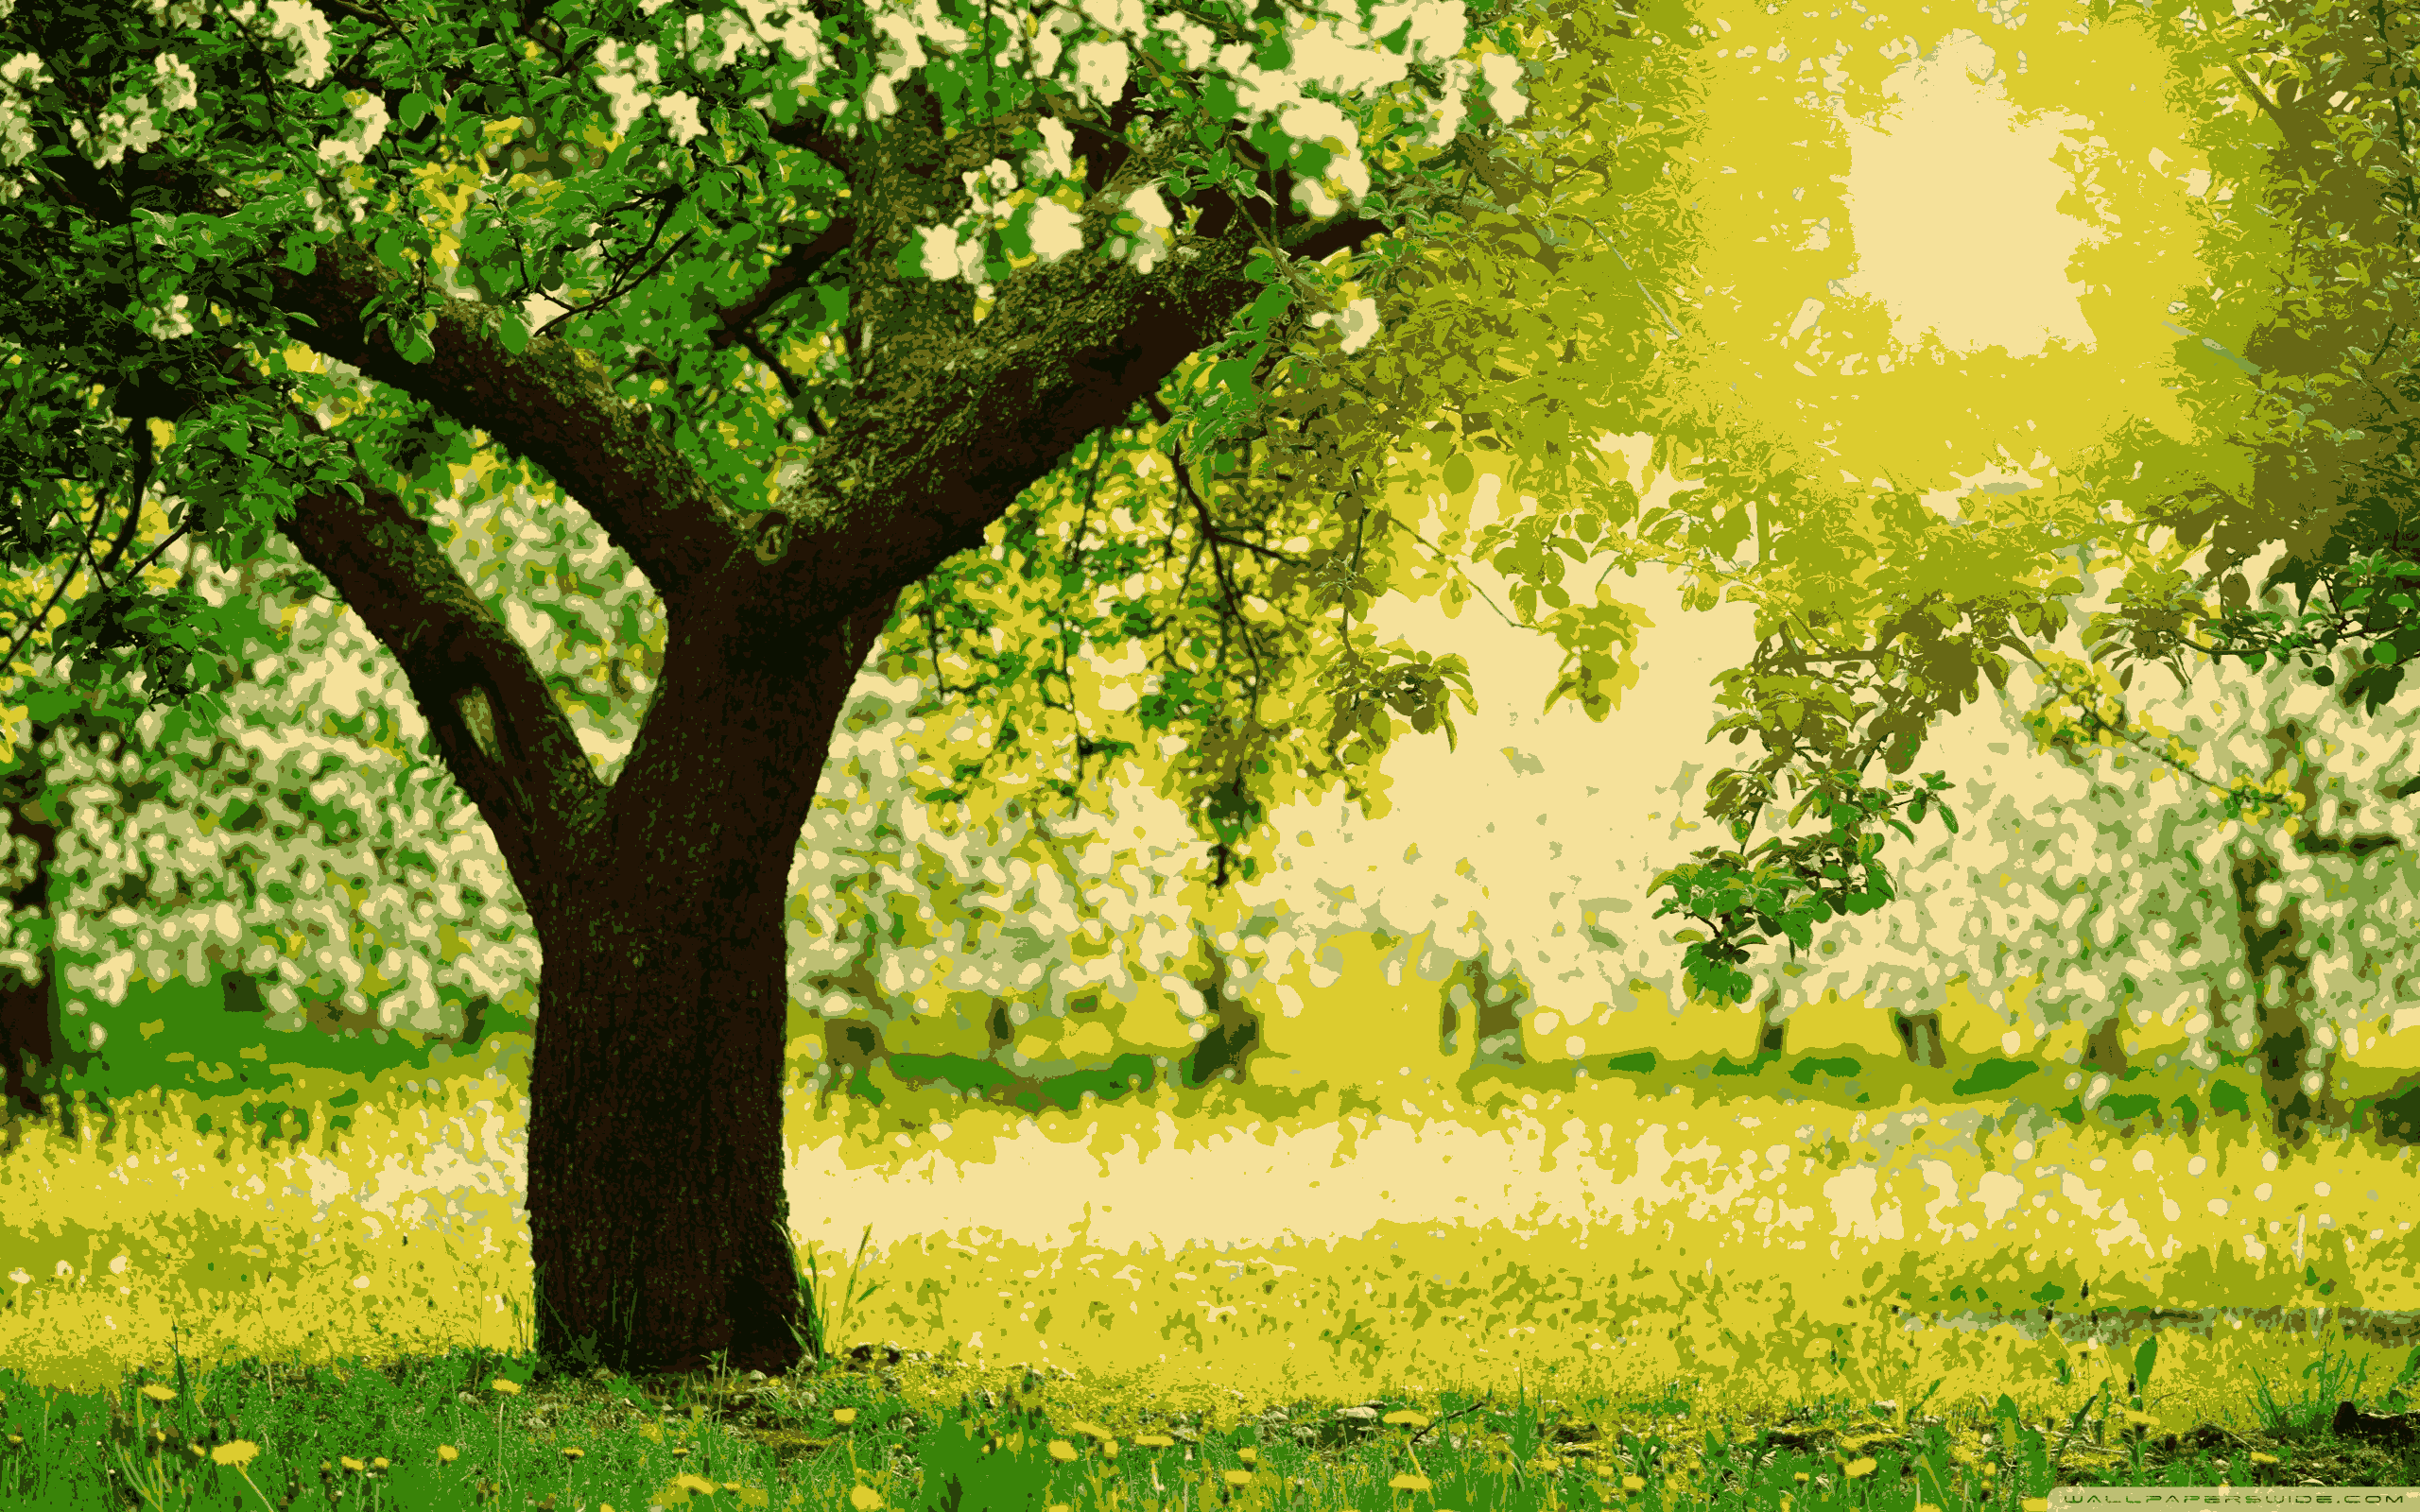
\includegraphics[width=\textwidth]{10Color}
        \caption{$K=10$}
        \label{fig:10COlor}
    \end{subfigure}
    \caption{Image Segmentation on 2560x1600 image}        
\end{figure}
\indent
The table below shows how file size of the original image is reduced.
\begin{center}
 \begin{tabular}{||c c||} 
 \hline
 K (Color) & File Size (KB) \\ [0.5ex] 
 \hline\hline
 Original Image & 1572  \\ 
 \hline
 10 & 1063 \\
 \hline
 7 & 742 \\
 \hline
 4 & 507  \\[1ex] 
 \hline
\end{tabular}
\end{center}
\section{Conclusion}
\indent
K-Means Algorithm could be very simple and quick to be implemented, the clustering problems where all clusters are centroids and separated can be solved by the algorithms. However, it will not be effective when the dataset and clusters are more complex.\\
\indent 
This report doesn't come with new idea to improve the effectiveness of the algorithm, the aim of the report is to introduce the reader to a basic, entry level clustering methods with some visual example on 2-dimensional and 3-dimensional dataset.

\section{Further research}
\indent
	The algorithm is simple to implement, however, the sensitivity to initial centroids, and strict structure of dataset, etc are those drawbacks of the algorithm which are undeniable . Further research could be made to improve the value of initial centroids. The traditional algorithm is depended on randomness, research could also be made to discover a way to make a fixed initial centroids. Furthermore, on a large dataset, the algorithm could be very slow to converge. Research could be spent to make the iteration stops earlier.
\section*{Acknowledgment}

The authors would like to thank Tiep V. Huu for useful machine learning blog and support, and also Prof. Andrew Ng for inspirational machine learning course on Coursera.

\begin{thebibliography}{2}

\bibitem{1}
Joaqun Prez Ortega, Ma. Del, Roco Boone Rojas, and Mara J.
Somodevilla \emph{"Research issues on k-means algorithm: An experimental trial using matlab"}.

\bibitem{2}
Arthur,~D.,~Vassilvitskii,~S., 2016. \emph{k-Means++: The Advantages of Careful Seeding.}Technical Report, Stanford.
\end{thebibliography}

\end{document}


